\section{Einführung und Ziele}
\subsection{Aufgabenstellung}
\textbf{Was ist PizzaPal?}
% \vspace{5pt}

PizzaPal ist eine Software zur Unterstützung der Lagerlogistik von Pizzerien, indem der Benutzer seine Zutaten über eine grafische Oberfläche verwaltet. Das Lager wird als zweidimensionaler Raum dargestellt, in dem ein Regal mit Paketen von Zutaten steht. \par
Ein Paket enthält Informationen zu Tragkraft, Maßen, Gewicht, Menge der Zutat und eine Liste von Unverträglichkeiten. Die Pakete werden in einer grafischen Oberfläche als Rechtecke in einer Regalstruktur verwaltet. Der Nutzer kann die Regale anpassen und Pakete hinzufügen, entfernen oder umorganisieren. Dabei dürfen keine Bretter überlastet werden und Unverträglichkeiten müssen berücksichtigt werden. Stapel von Paketen müssen ebenfalls verwaltet und verschoben werden können.\par
Fehler beim Erstellen oder Umlagern von Paketen und bei der Regalkonfiguration sollen dem Nutzer grafisch angezeigt werden. Für spezifizierte Anwendungsfälle siehe Anforderungsdokument (V1.1). In der nachfolgenden Tabelle sind die Anforderung absteigend priorisiert aufgelistet.

\begin{figure}[H]
    \label{fig:funktionaleAnforderungenTabelle}
    \begin{longtable}{|m{0.3\textwidth}|m{0.7\textwidth}|}
        \hline
        \textbf{Anforderung} & \textbf{Erklärung} \\
        \hline
        Paketvorlage anlegen & Eine Vorlage für ein Paket einer bestimmten Zutat, mit dem dazugehörigen Gewicht, der Tragkraft, den Maßen des Pakets und der Menge an Inhalt anlegen \\
        \hline
        Brett- und Stützenvorlage erzeugen & Vorlagen für Bretter und Stützen anlegen \\
        \hline
        Bretter und Stützen erzeugen & Bretter- und Stützenobjekte aus Vorlagen erstellen \\
        \hline
        Regal hinzufügen & In einem leeren Lagerraum ein neues Regal bauen \\
        \hline
        Pakete erzeugen & Ein Paket aus einem Template erzeugen und platzieren \\
        \hline
        Pakete anordnen & Ein Paket im Regal per Drag\&Drop an einen anderen Ort verschieben \\
        \hline
        Pakete validieren & Ein Paket wenn es platziert wird auf Verträglichkeiten mit benachbarten Paketen testen \\
        \hline
        Paketvorlage bearbeiten & Das Gewicht, Tragkraft, Menge oder Maße einer Paketvorlage ändern \\
        \hline
        Pakete löschen & Ein Paket im Regal löschen \\
        \hline
        Bestehende Bretter und Stützen anpassen & Bretter und Stützen die bereits existieren anpassen \\
        \hline
        Bestehende Bretter und Stützen bewegen & Bretter und Stützen im Raum bewegen \\
        \hline
        Regal bearbeiten & Ein bereits bestehendes Regal umbauen \\
        \hline
        Inventarliste anzeigen & Zeigt eine nach Zutaten sortierte Liste der in einem Regal vorhandenen Pakete an \\
        \hline
    \end{longtable}
    % \captionbelow[Tabelle]{Funktionale Anforderungen an PizzaPal}
\end{figure}

\begin{figure}[H]
    \captionabove{Beispiel für die GUI}
    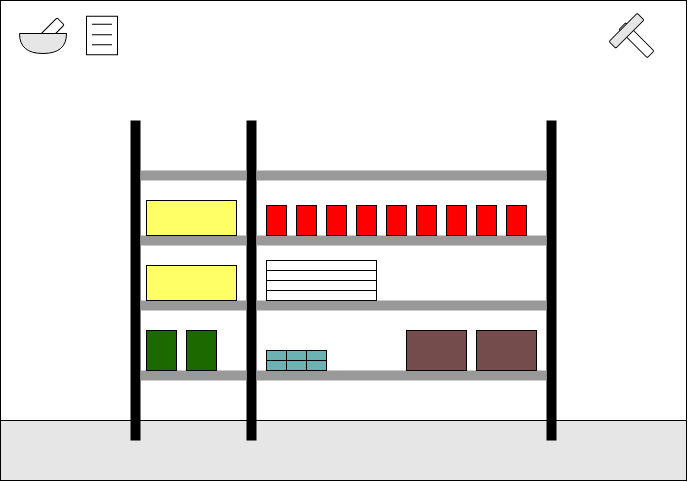
\includegraphics[width=\linewidth]{./images/einfuehrung/GUI-Skizze.png}
    \label{fig:GUIbeispiel}
\end{figure}

\newpage
\subsection{Qualitätsziele}
Die folgende Tabelle beschreibt die zentralen Qualitätsziele von PizzaPal. Die Reihenfolge gibt eine grobe Orientierung bezüglich der Priorisierung vor. Für weitere Details siehe Rahmenbedingungen \& Technische Anforderungen im Anforderungsdokument(Version 1.1).

\begin{longtable}{|m{0.3\textwidth}|m{0.7\textwidth}|}
    \hline
    \textbf{Qualitätsziel} & \textbf{Motivation und Erläuterung} \\
    \hline
    Benutzerfreundlichkeit & Das System muss eine intuitive und einfache Bedienung ermöglichen, insbesondere durch die Verwendung von Drag\&Drop für die Anordnung der Regale und Pakete. \\
    \hline
    Zuverlässigkeit & Das System muss sicherstellen, dass keine Regalböden überlastet werden und keine Pakete mit Unverträglichkeiten zusammen gelagert werden. \\
    \hline
    Leistung & Das Programm soll schnell reagieren, insbesondere beim Laden und Anordnen von Paketen sowie beim Umbauen der Regale. \\
    \hline
    Skalierbarkeit & Das System muss in der Lage sein, verschiedene Größen und Mengen an Paketen und Regalen zu verwalten, ohne die Leistung zu beeinträchtigen. \\
    \hline
    Kompatibilität & Das Programm muss mindestens unter der aktuellen Kubuntu 22.04.4 LTS Linux-Version funktionieren und die technischen Anforderungen erfüllen (Java 21, 8 GB RAM, Full-HD Bildschirm, Maus). \\
    \hline
    Grafische Darstellung & Die grafische Benutzeroberfläche muss klar und übersichtlich sein, Fehler und Unverträglichkeiten müssen deutlich angezeigt werden. \\
    \hline
\end{longtable}

\newpage
\subsection{Stakeholder}

\begin{longtable}{|m{0.3\textwidth}|m{0.7\textwidth}|}
    \hline
    \textbf{Stakeholder} & \textbf{Interesse, Bezug} \\
    \hline
    Pizzeriapersonal & Die Hauptnutzer der Software, die die Zutaten im Lager verwalten müssen, für das Anlegen, Bearbeiten und Organisieren der Lagerregale und Pakete verantwortlich sind oder die gelegentlich das Lager verwalten oder Inventuren durchführen müssen.\\
    \hline
    Software-Entwickler & Personen, die das System entwickeln und warten. \\
    \hline
    Geschäftsleitung der Pizzeria & Interessenten an einer effizienten und fehlerfreien Lagerverwaltung zur Kostenoptimierung und Verbesserung der Betriebsabläufe. \\
    \hline
    IT-Support & Zuständig für die technische Unterstützung und Wartung der Software. \\
    \hline
\end{longtable}